\newcommand{\anhangText}{
	% Gibt es nicht
}

\newcommand{\anhangEins}{
	\begin{figure}[h!]
		\centering
		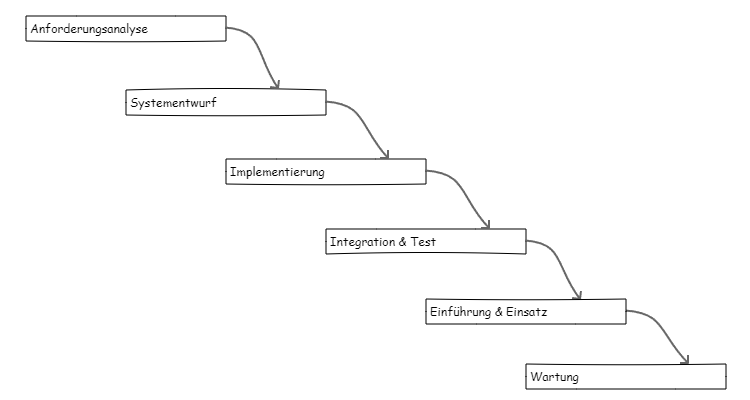
\includegraphics[width=13cm]{img/Wasserfallmodell.png}
		\caption{Darstellung des geplanten Wasserfall-Modells}
		\label{fig:wasserfallmodell}
	\end{figure}
}

\newcommand{\anhangZwei}{
	\paragraph{To-Dino Appliklation}
	\begin{figure}[h!]
		\centering
		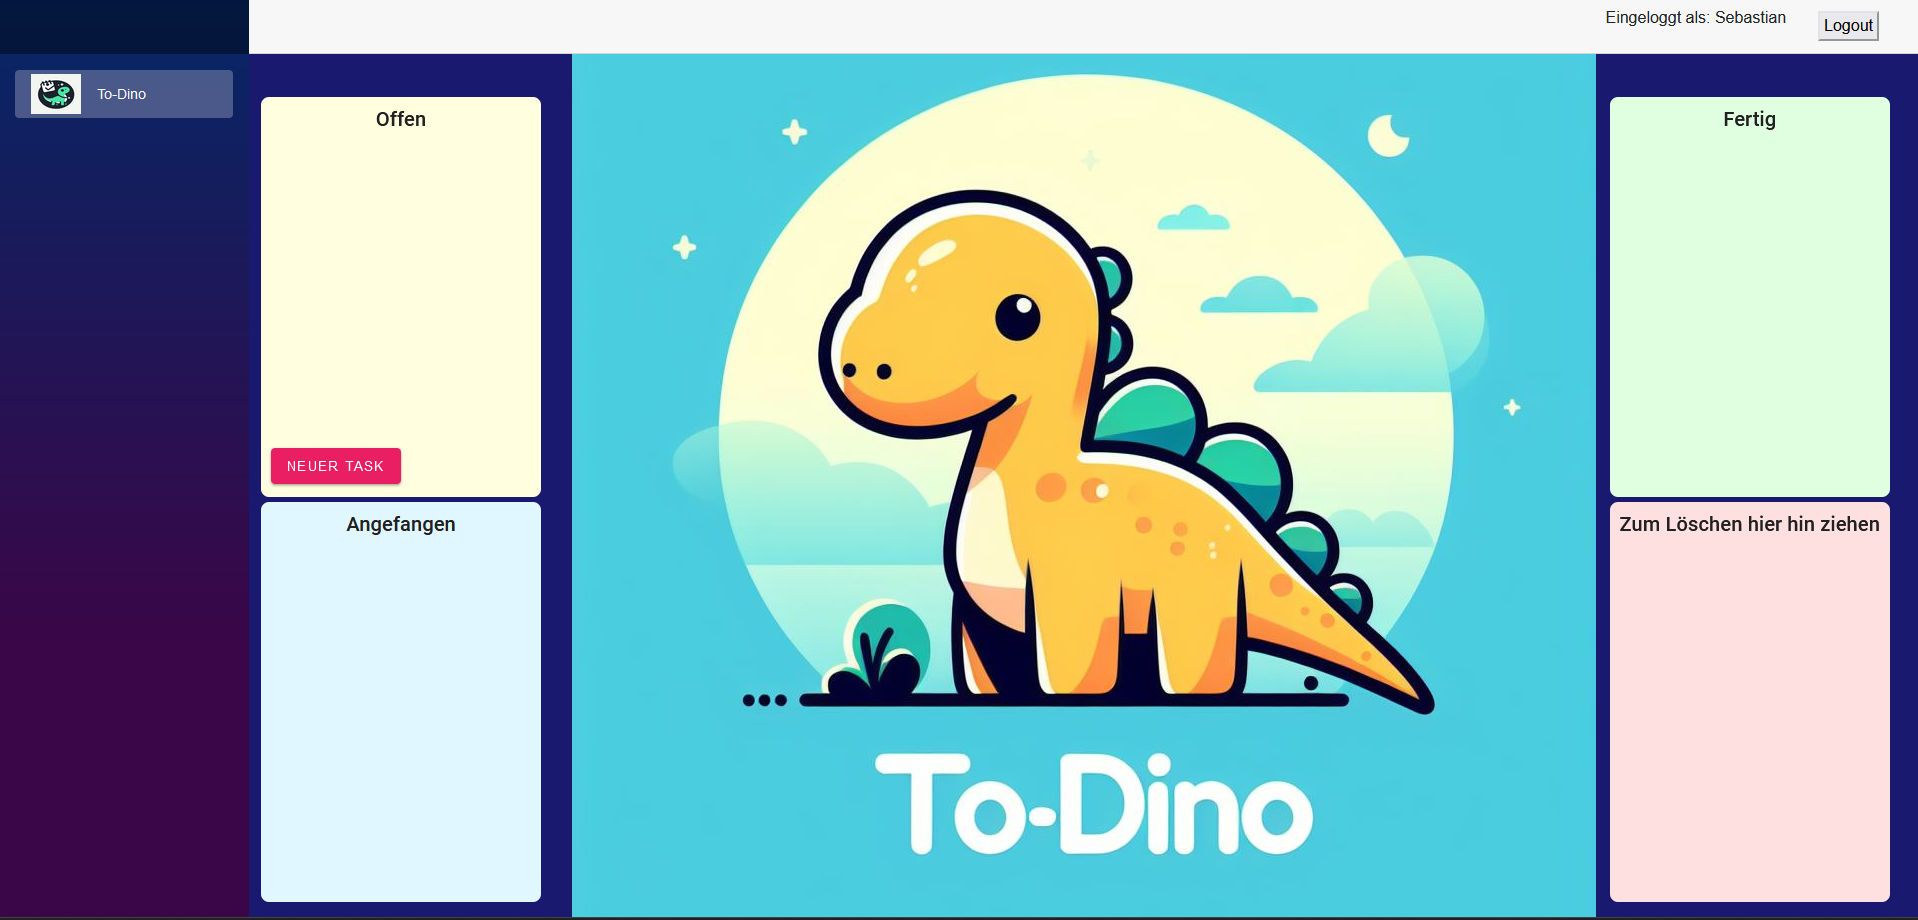
\includegraphics[width=13cm]{img/ToDino.png}
		\caption{To-Dino Applikation}
		\label{fig:todinoapp}
	\end{figure}
	
}

\newcommand{\anhangDrei}{
	\paragraph{ApplicationDbContext}
	\begin{figure}[h!]
		\centering
		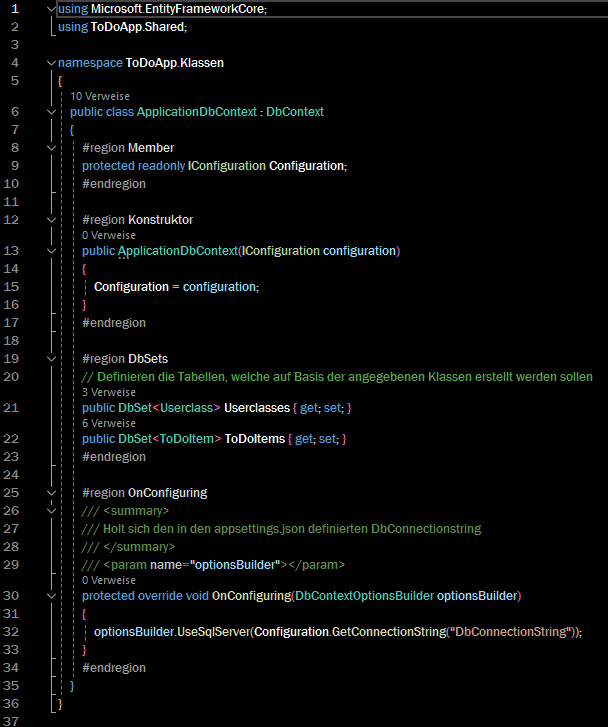
\includegraphics[width=13cm]{img/ApplicationDbContext.png}
		\caption{ApplicationDbContext.cs}
		\label{fig:applicationdbcontext}
	\end{figure}
}

\newcommand{\anhangVier}{
	\paragraph{Datenbank Init-File}
	\begin{figure}[ht]
		\centering
		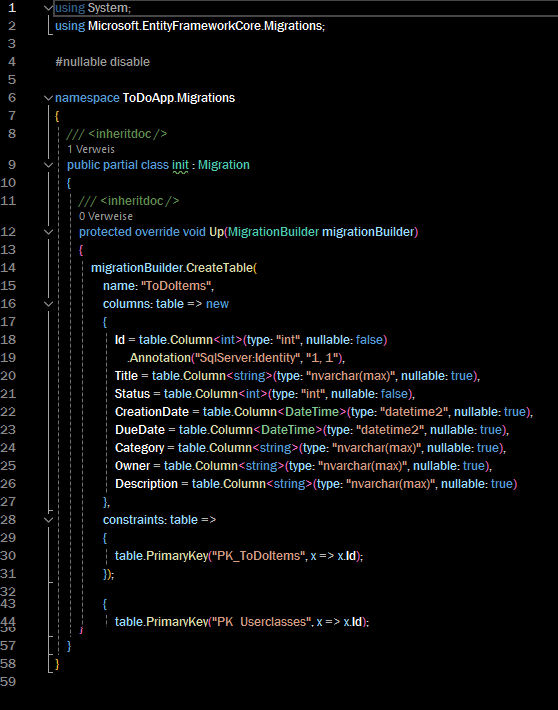
\includegraphics[width=13cm]{img/Db_Init_File.png}
		\caption{Generierte Init-File für die Datenbankerstellung}
		\label{fig:dbinitfile}
	\end{figure}
}

\newcommand{\anhangFuenf}{
	\paragraph{Datenbank Migration Snapshot}
	\begin{figure}[ht]
		\centering
		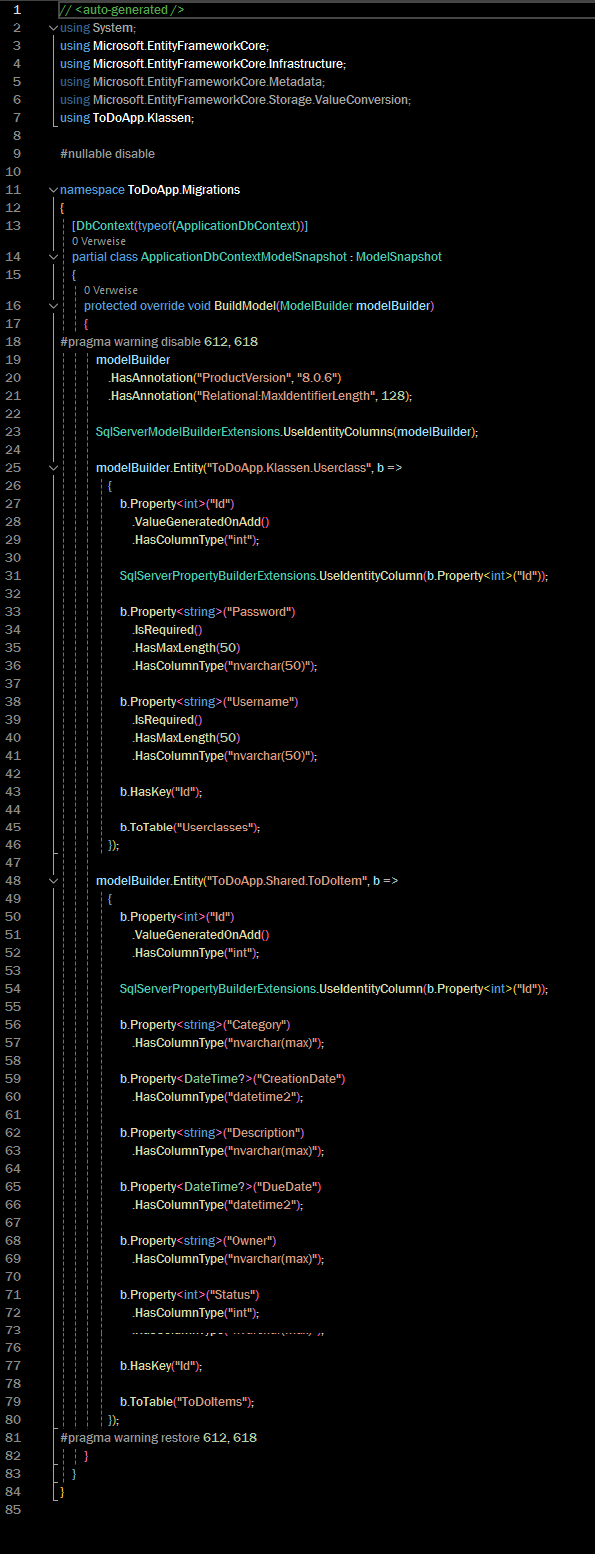
\includegraphics[width=13cm]{img/Db_Migration_Snapshot.png}
		\caption{Generierter Datenbank-Migration-Snapshot}
		\label{fig:dbmigrationsnapshot}
	\end{figure}
}

\newcommand{\anhangSechs}{
	\paragraph{Login Modal Dialog}
	\begin{figure}[ht]
		\centering
		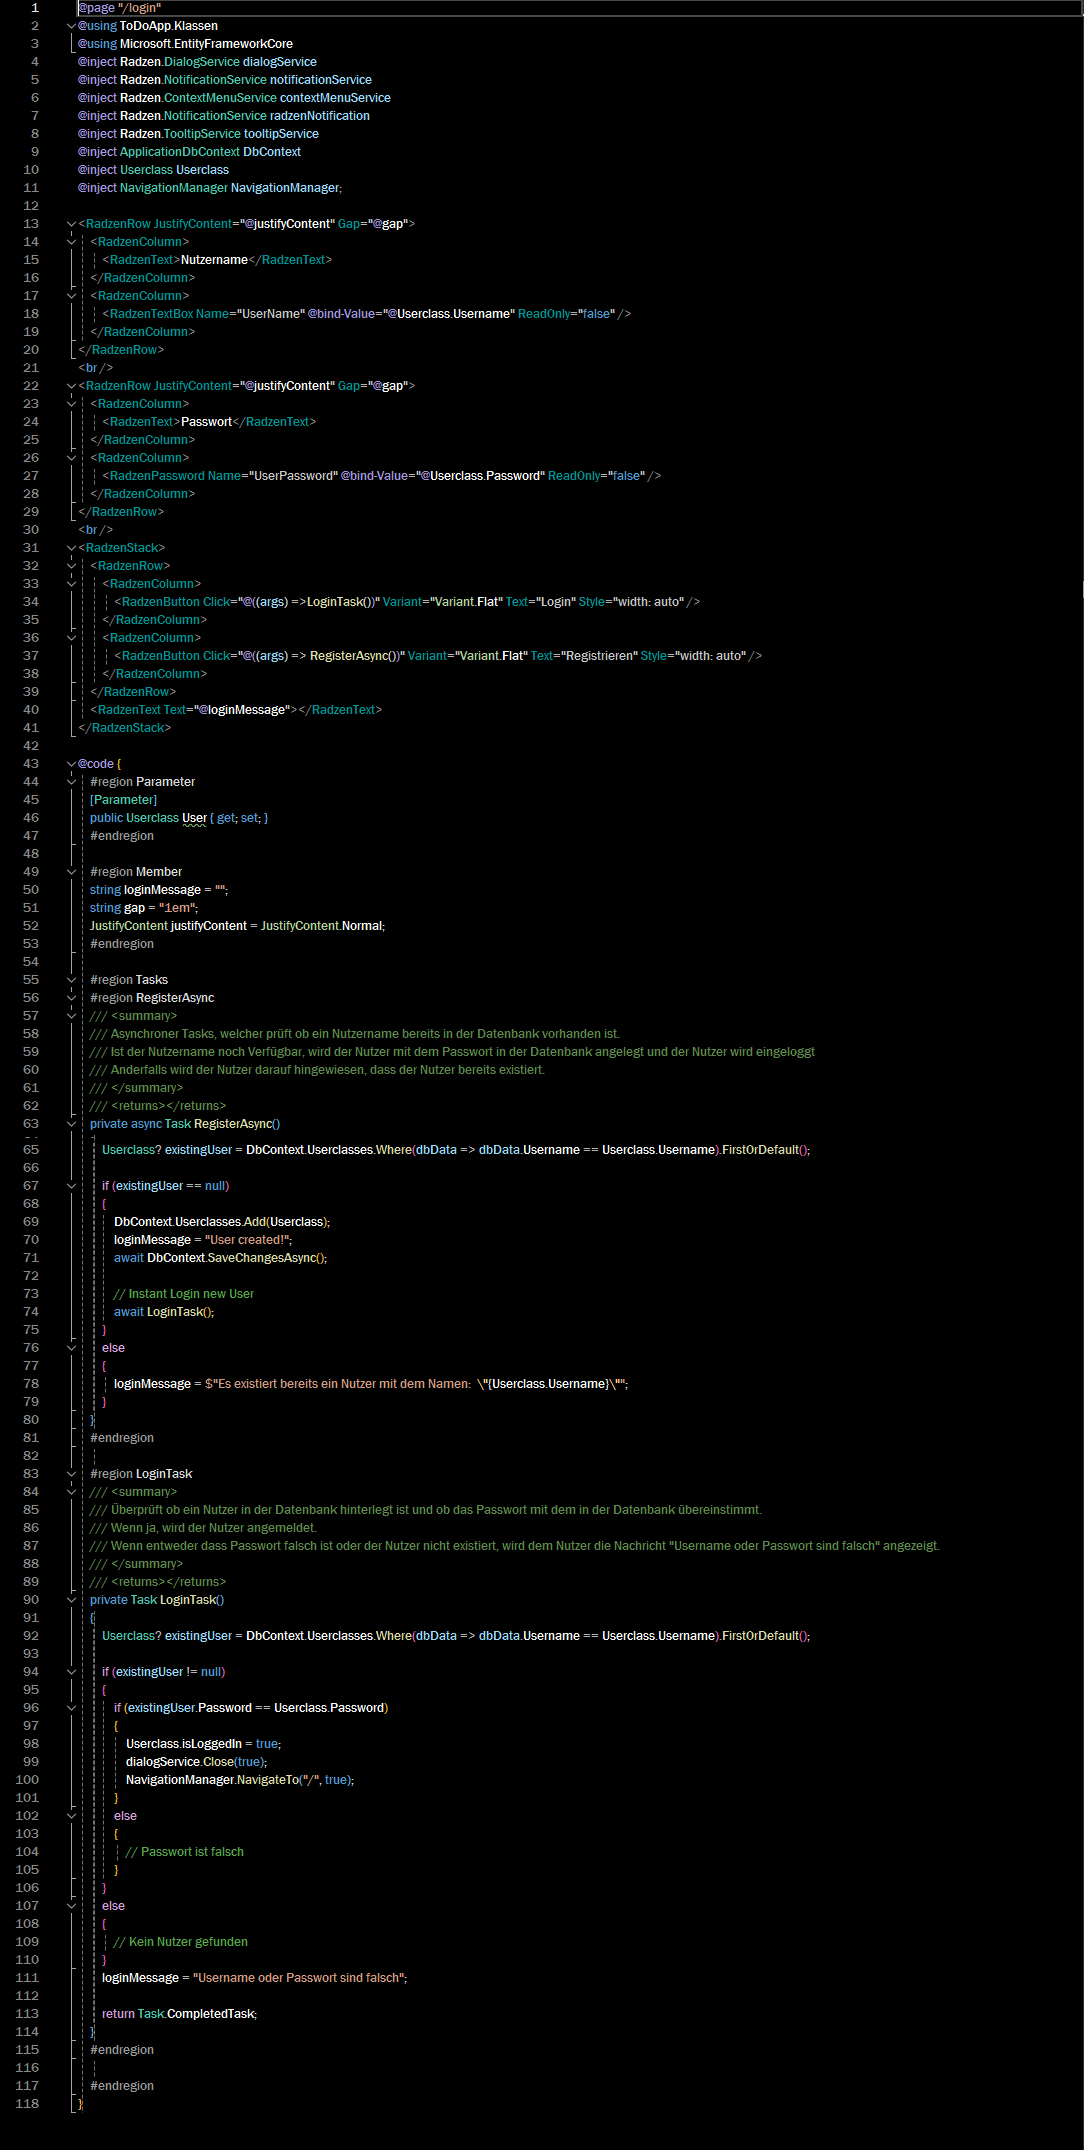
\includegraphics[width=13cm]{img/LoginModal.png}
		\caption{LoginModal.cs}
		\label{fig:loginmodal}
	\end{figure}
}

\newcommand{\anhangSieben}{
	\paragraph{ToDoItem-Klasse}
	\begin{figure}[ht]
		\centering
		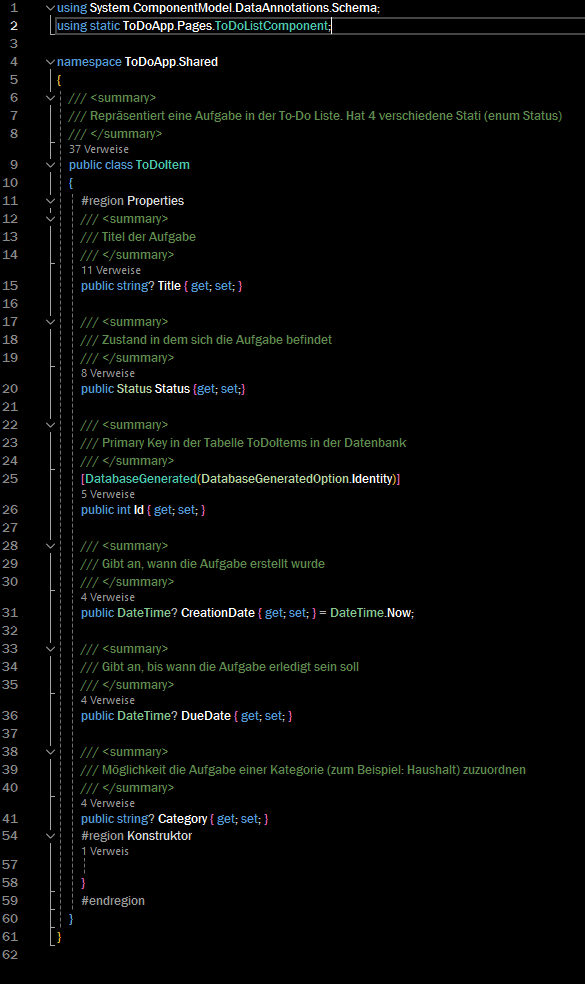
\includegraphics[width=13cm]{img/ToDoItem.png}
		\caption{ToDoItem.cs}
		\label{fig:todoitemklasse}
	\end{figure}
}

\newcommand{\anhangAcht}{
	\paragraph{ToDoItem Modaldialog}
	\begin{figure}[ht]
		\centering
		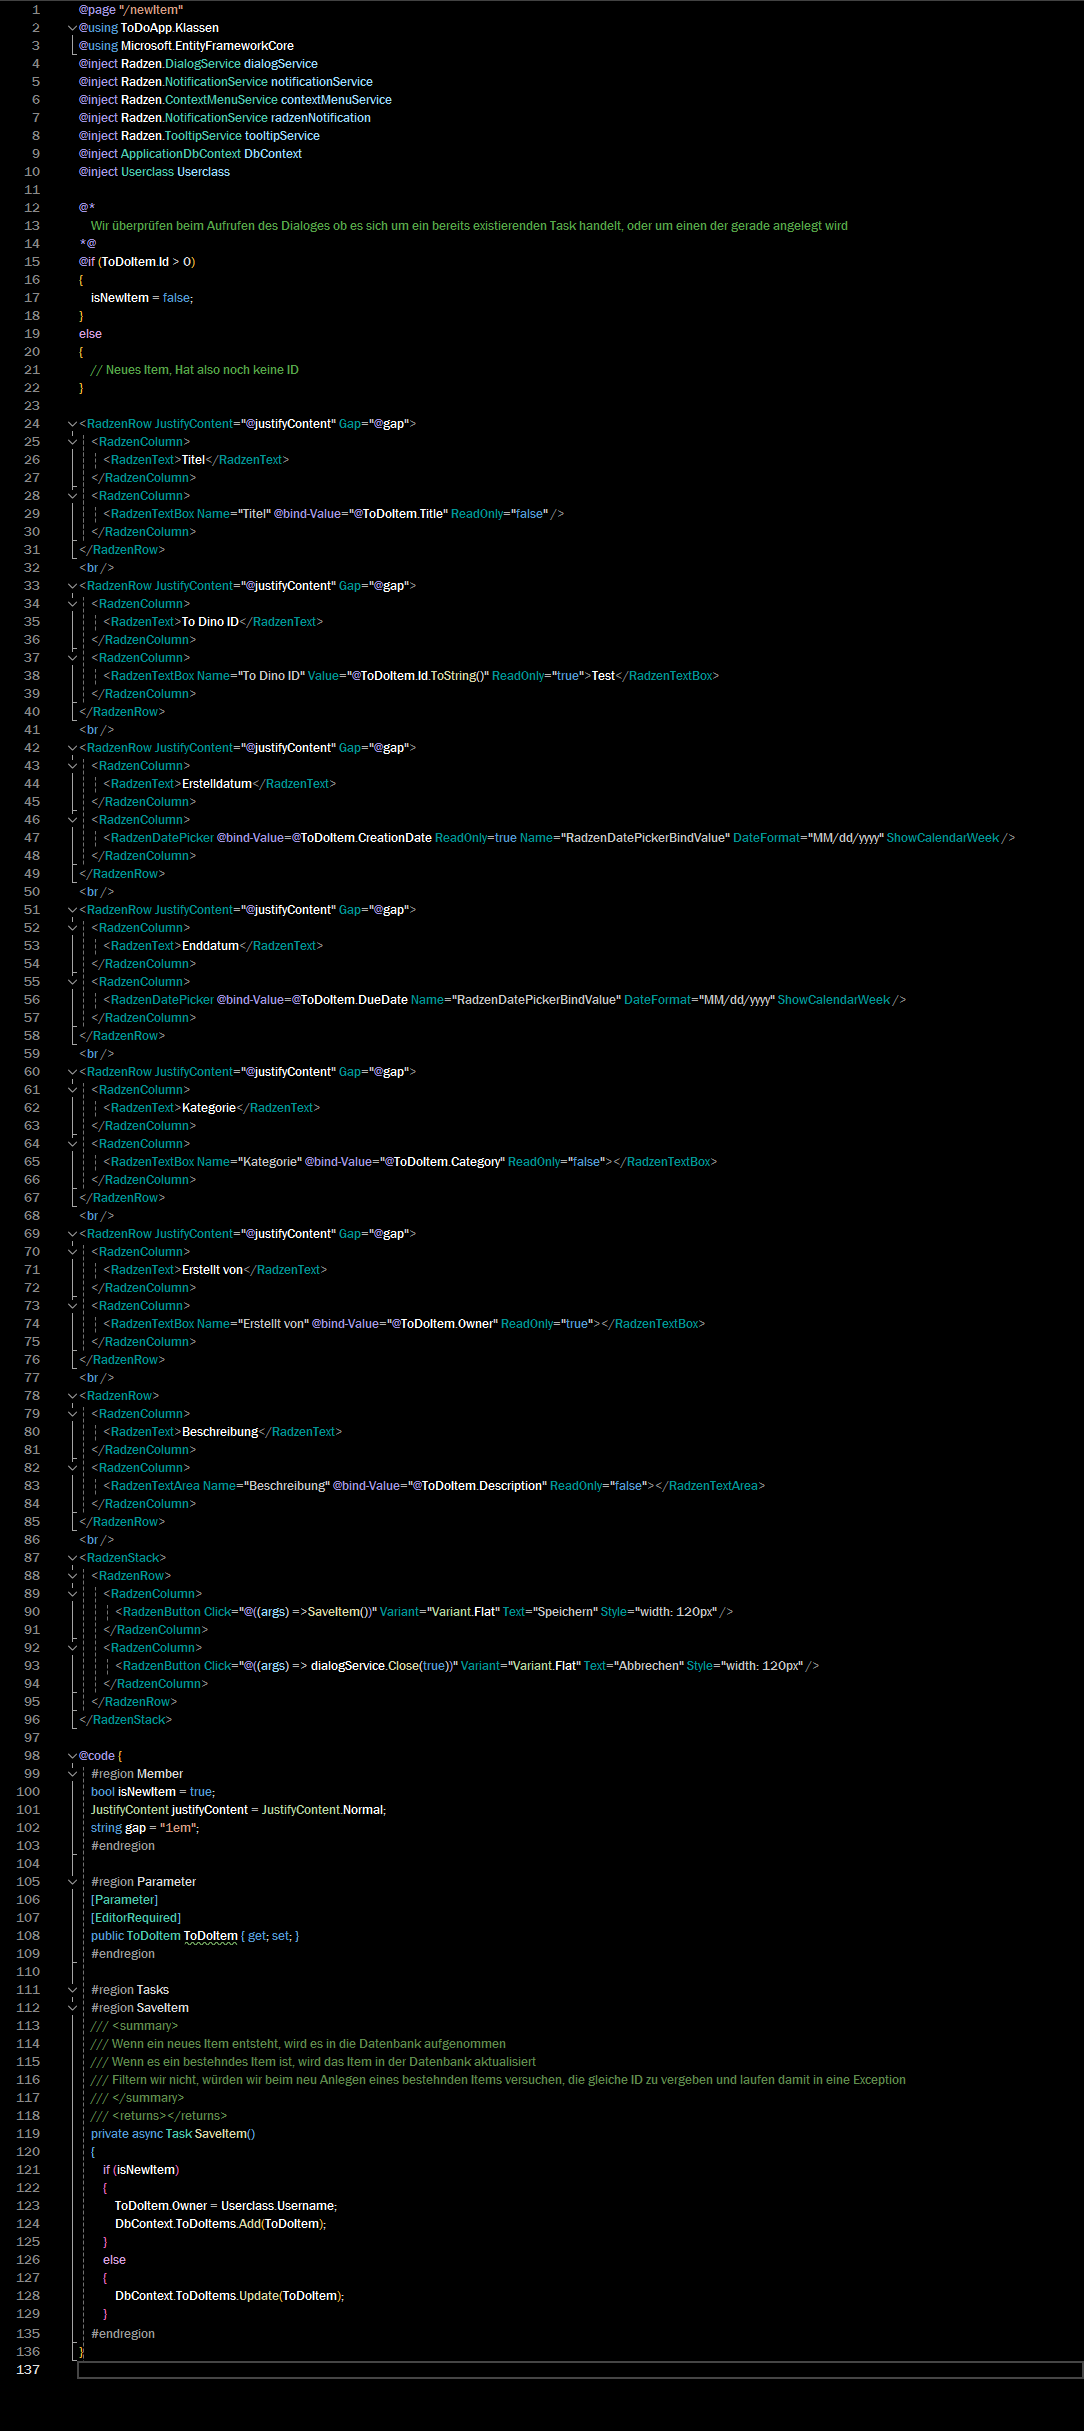
\includegraphics[width=13cm]{img/ToDoItemModal.png}
		\caption{ToDoItemModal.cs}
		\label{fig:todoitemmodal}
	\end{figure}
}

\newcommand{\anhangNeun}{
	\paragraph{ToDoListComponent-Komponente}
	\begin{figure}[ht]
		\centering
		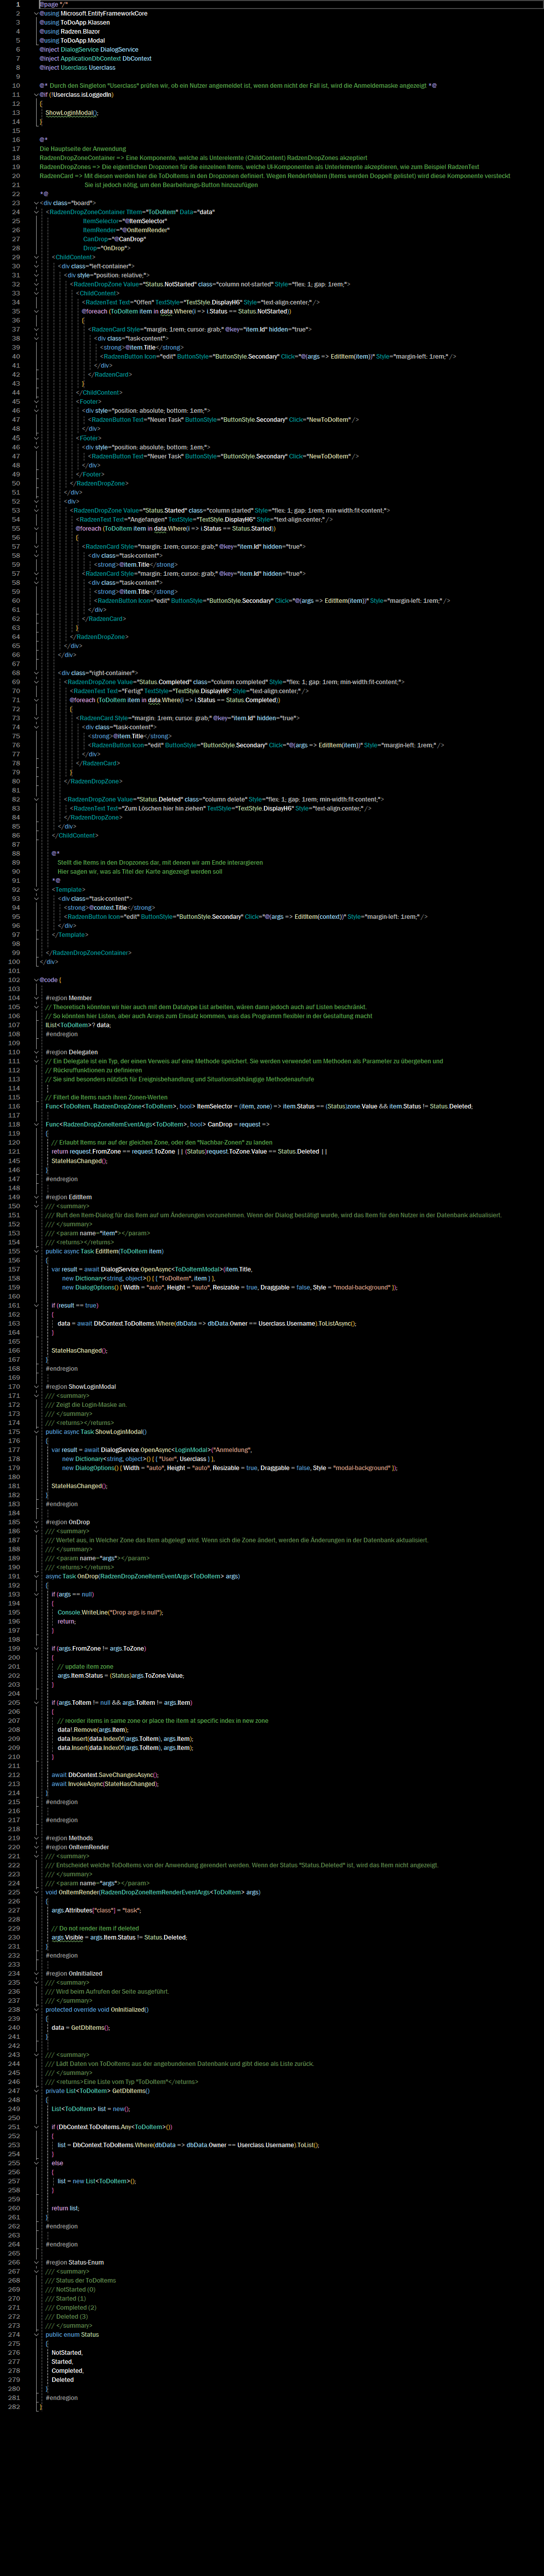
\includegraphics[width=13cm]{img/ToDoListComponent.png}
		\caption{ToDoListComponent.cs}
		\label{fig:todolistcomponent}
	\end{figure}
}

\newcommand{\anhangZehn}{
	\paragraph{Userclass-Klasse}
	\begin{figure}[ht]
		\centering
		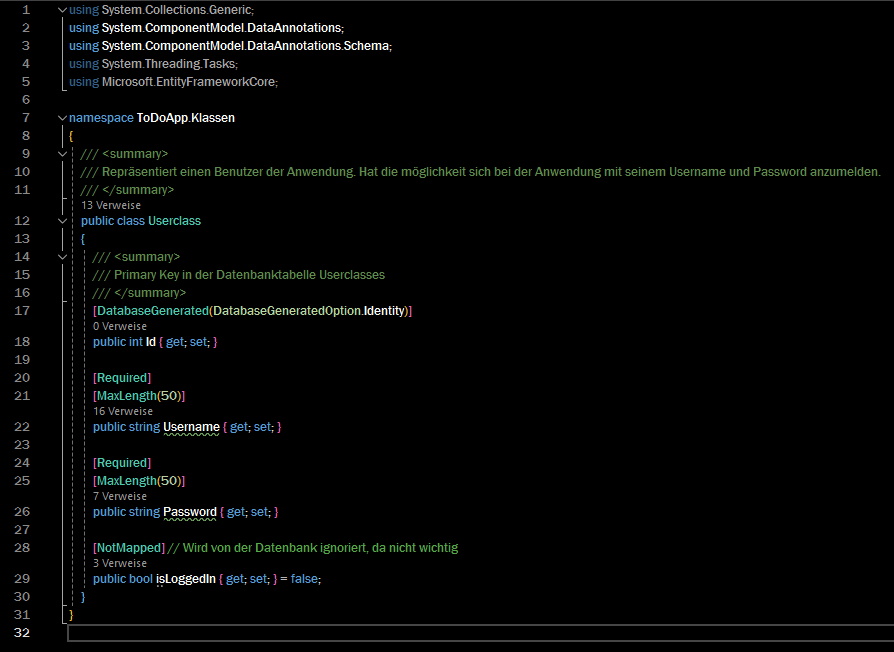
\includegraphics[width=13cm]{img/Userclass.png}
		\caption{Userclass.cs}
		\label{fig:Userclass}
	\end{figure}
}

\newcommand{\anhangElf}{
	\paragraph{To-Dino Mockup}
	\begin{figure}[ht]
		\centering
		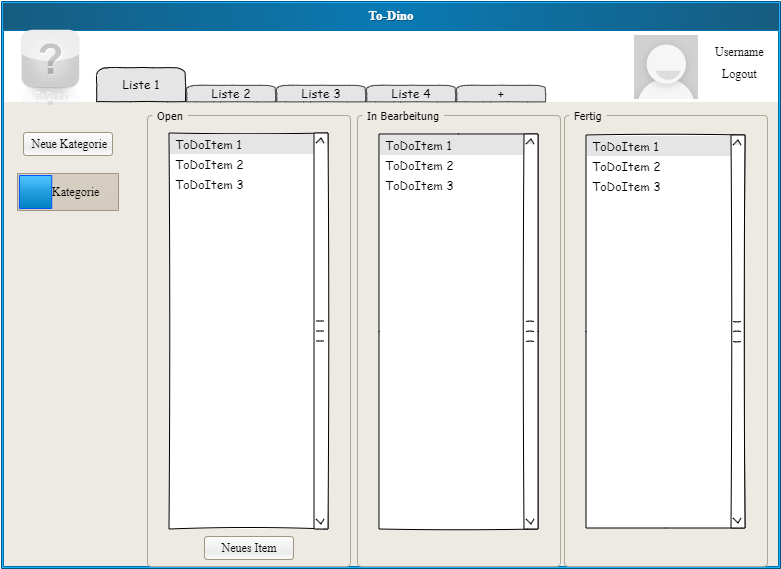
\includegraphics[width=13cm]{img/ToDinoMockup.png}
		\caption{To-Dino Mockup}
		\label{fig:todinomockup}
	\end{figure}
}

\newcommand{\anhangZwoelf}{
	\paragraph{ToDoItem Modaldialog Mockup}
	\begin{figure}[ht]
		\centering
		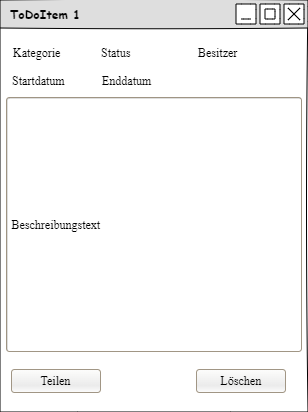
\includegraphics[width=13cm]{img/ToDoItemModalMockup.png}
		\caption{ToDoItem Modaldialog Mockup}
		\label{fig:todoitemmodalmockup}
	\end{figure}
}